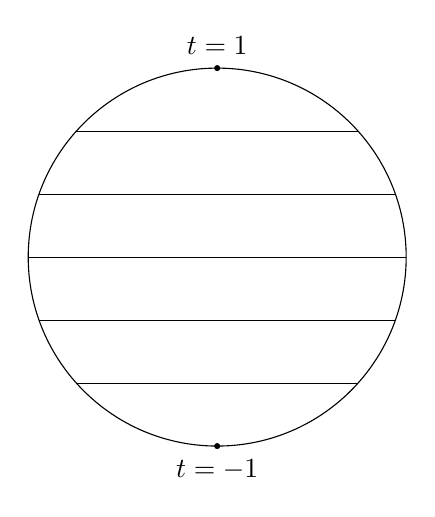
\begin{tikzpicture}[line cap=round]
    \tikzset{pole/.style={circle, fill=black, inner sep=0pt, minimum size=2.2pt}}
  % parameters
  \def\R{2.4}      % radius (cm)
  \def\N{5}        % number of chords

  % compute spacing so chords don't sit on the boundary
  \pgfmathsetmacro{\step}{2*\R/(\N+1)}

  % draw chords inside the circle
  \begin{scope}
    \clip (0,0) circle (\R);
    \foreach \i in {1,...,\N} {
      \draw (-\R-0.3, -\R + \i*\step) -- (\R+0.3, -\R + \i*\step);
    }
  \end{scope}

  % circle outline last so it sits on top
  \draw (0,0) circle (\R);

  \node[pole, label={above:$t=1$}]   at (0,\R)   {};
  \node[pole, label={below:$t=-1$}]  at (0,-\R)  {};
\end{tikzpicture}
